%
\documentclass[10pt,a4paper]{article}


\usepackage{array}
\usepackage{subfigure}
\usepackage{graphicx}
\usepackage{amssymb}
\usepackage{amsmath}
\usepackage{cite}
\usepackage{color}
\usepackage{url}
\usepackage[lined,linesnumbered,ruled,norelsize]{algorithm2e}
\usepackage{listings}
\lstset{
  language=Octave, 
  basicstyle=\footnotesize, 
  frame=single, 
  showspaces=false, 
  showstringspaces=false}




\begin{document}

\title{Experiment 2: Logistic Regression and Newton's Method}

\maketitle
  
\section{Description}
%
  In this exercise, you will use Newton's Method to implement logistic regression on a classification problem.



\section{Data}
%
  To begin, download data2.zip and extract the files from the zip file. For this exercise, suppose that a high school has a dataset representing 40 students who were admitted to college and 40 students who were not admitted. Each $(x^{(i)}, y^{(i)})$ training example contains a student's score on two standardized exams and a label of whether the student was admitted.

  Your task is to build a binary classification model that estimates college admission chances based on a student's scores on two exams. In your training data, the first column of your $x$ array represents all Test 1 scores, and the second column represents all Test 2 scores, and the $y$ vector uses ``1'' to label a student who was admitted and ``0'' to label a student who was not admitted.




\section{Plot the Data}
%
  Load the data for the training examples into your program and add the $x_0 = 1$ intercept term into your x matrix.

  Before beginning Newton's Method, we will first plot the data using different symbols to represent the two classes. In Matlab/Octave, you can separate the positive class and the negative class using the find command:
  %
  \begin{lstlisting}
    % find returns the indices of the
    % rows meeting the specified condition
    pos = find(y == 1); neg = find(y == 0);

    % Assume the features are in the 2nd and 3rd
    % columns of x
    plot(x(pos, 2), x(pos,3), '+'); hold on
    plot(x(neg, 2), x(neg, 3), 'o')
  \end{lstlisting}
  %
  Your plot should look like the following:
  %
  \begin{figure}[htb!]
    \centering
      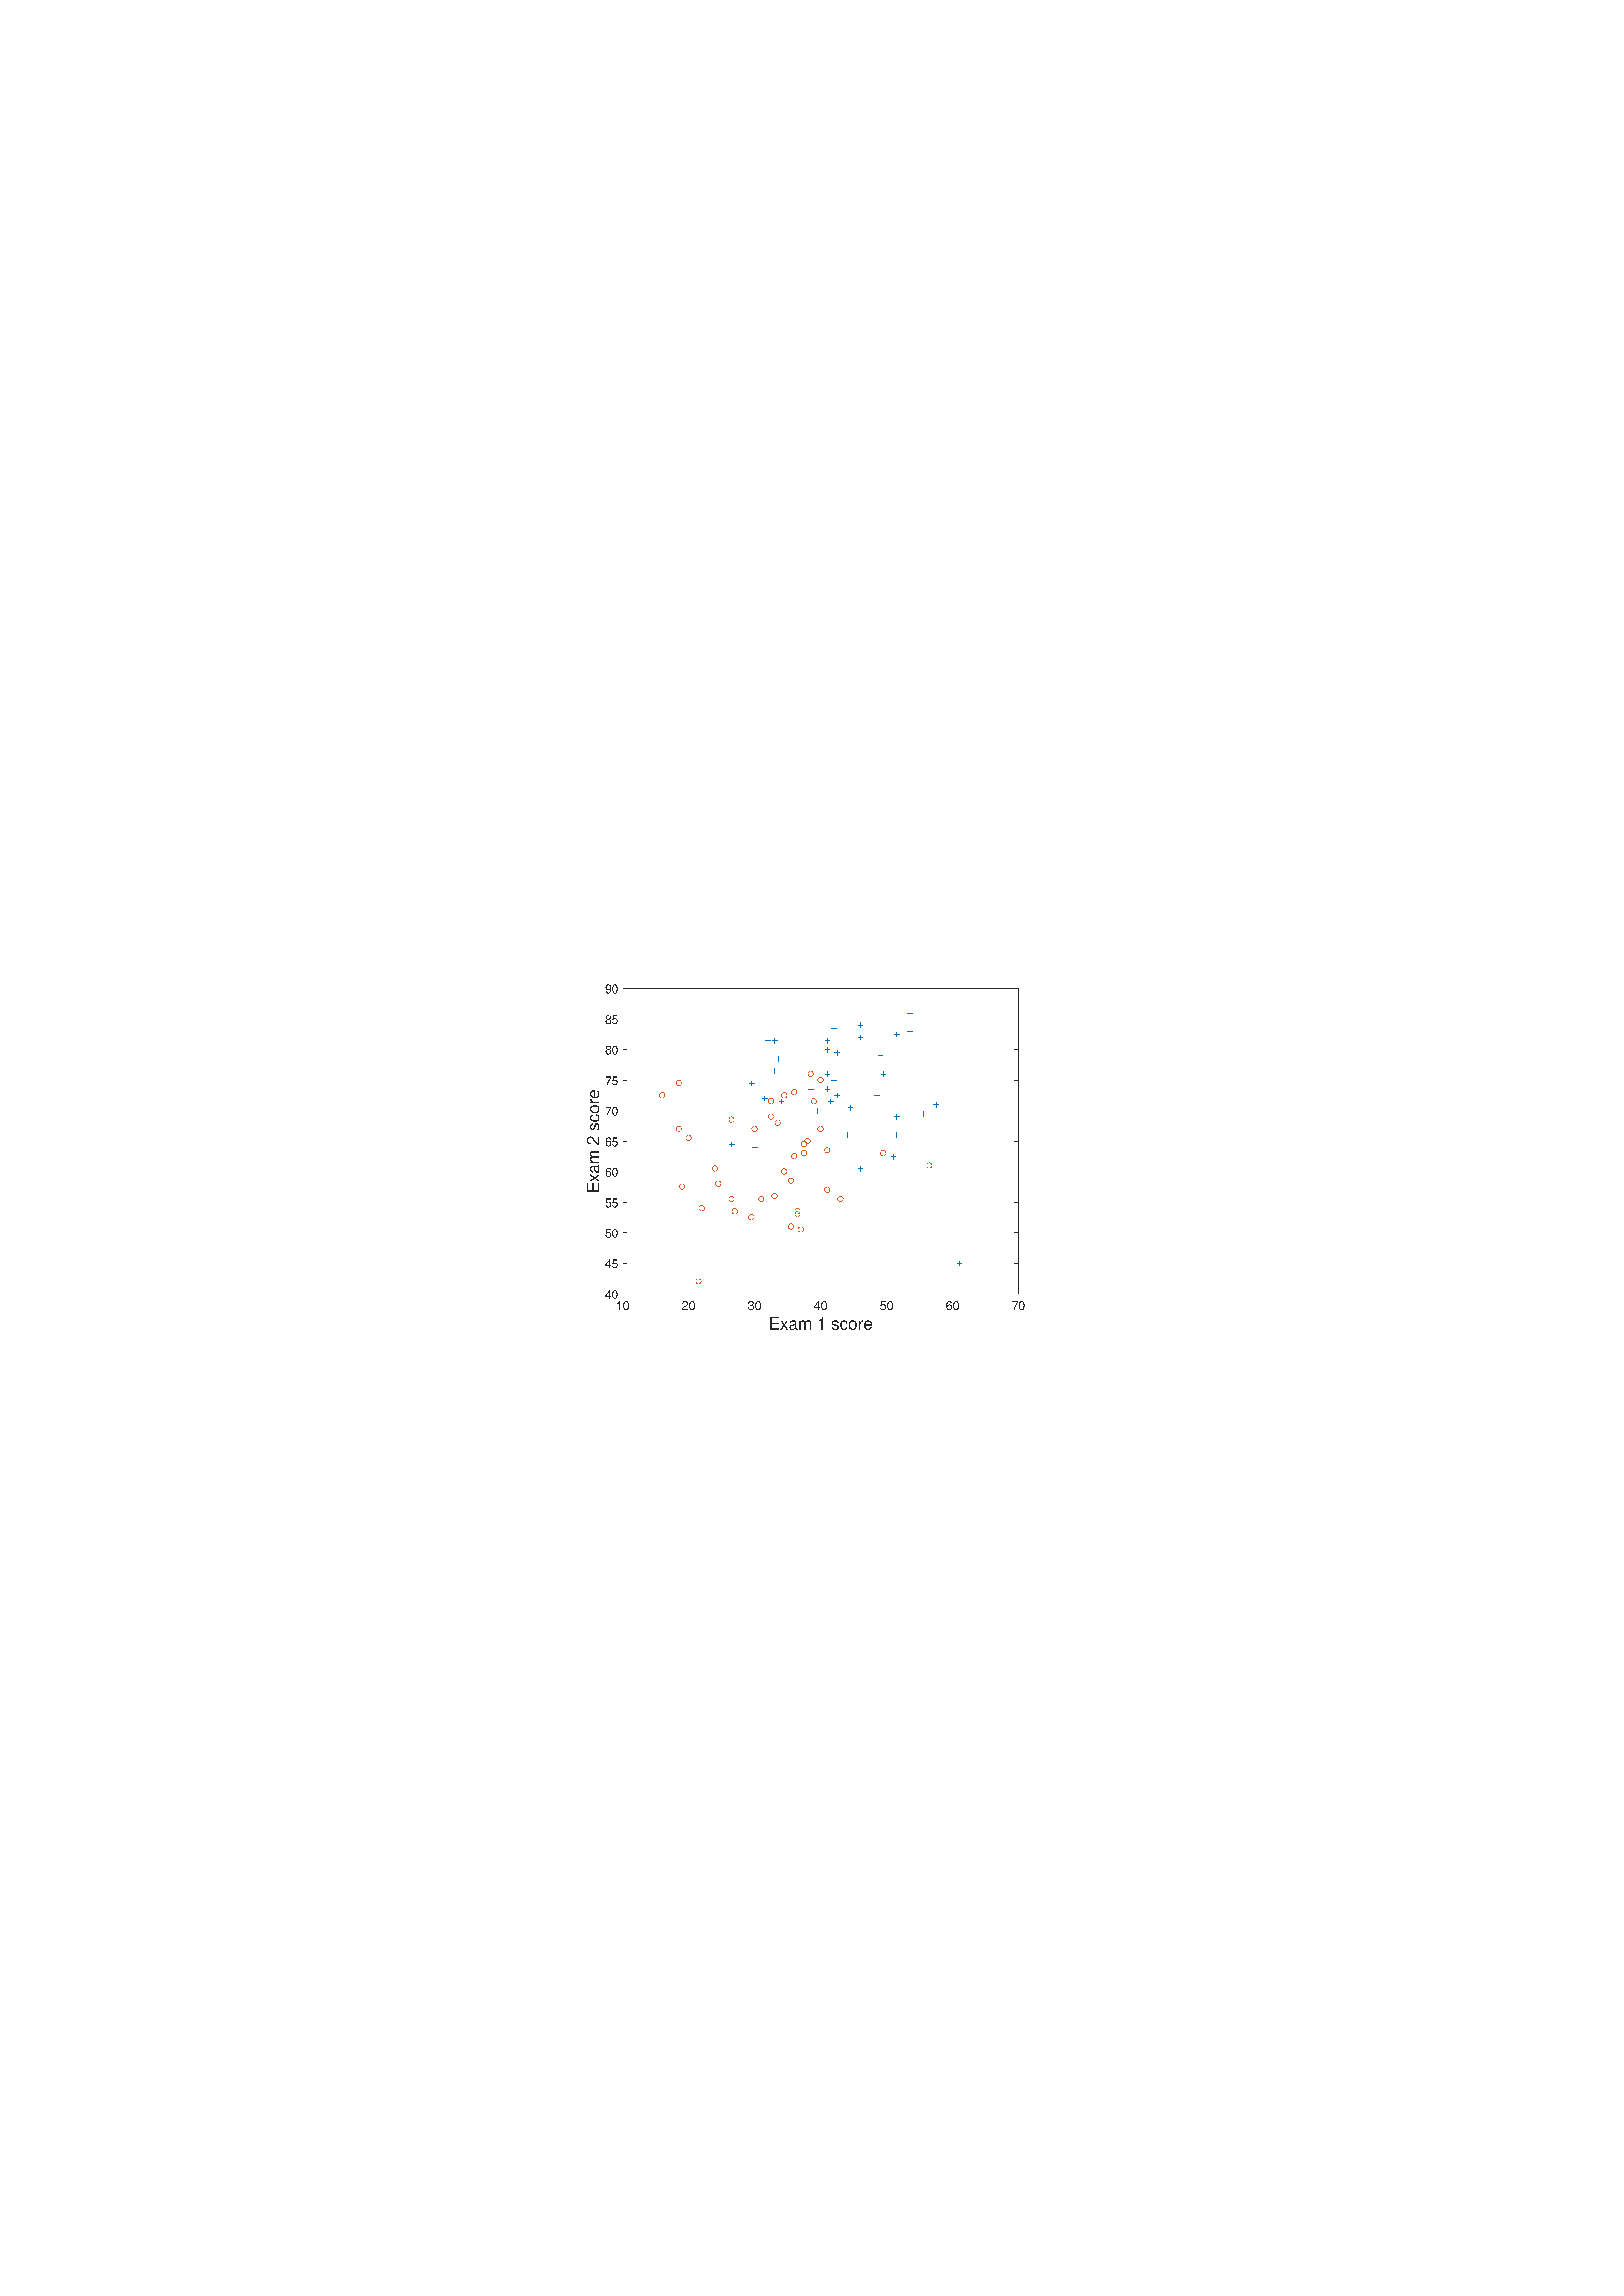
\includegraphics[width=.7\columnwidth]{datasamples}
  \end{figure}





\section{Logistic Regression}
%
  Recall that in logistic regression, the hypothesis function is 
  %
  \begin{equation}
    h_\theta(x) = g(\theta^T x) = \frac{1}{1+e^{-\theta^T x}} = P(y=1 \mid x; \theta) 
  \end{equation}
  %
  Matlab/Octave does not have a library function for the sigmoid, so you will have to define it yourself. The easiest way to do this is through an inline expression:
  %
  \begin{lstlisting}[language=Octave, basicstyle=\footnotesize, showspaces=false]
    g = inline('1.0 ./ (1.0 + exp(-z))'); 
    % Usage: To find the value of the sigmoid 
    % evaluated at 2, call g(2)
  \end{lstlisting}




  Given a set of training data $\{x^{(i)}\}_{i=1,\cdots,m}$, we define a likelihood function as
  %
  \begin{equation}
    J(\theta) = \prod^m_{i=1} (h_\theta(x^{(i)}))^{y^{(i)}} (1-h_\theta (x^{(i)}))^{1-y^{(i)}}
  \end{equation}
  %
  To facilitate the computation, we maximize the following log likelihood function
  %
  %
  \begin{equation}
    L(\theta) = \frac{1}{m} \sum^m_{i=1} [ y^{(i)} \log(h_\theta(x^{(i)})) + (1-y^{(i)}) \log (1 - h_\theta(x^{(i)}))  ]
  \label{eq:lh}
  \end{equation}  
  %
  %
  Note that maximizing (\ref{eq:lh}) is equivalent to minimizing its negative. Then, our problem becomes \footnote{Note that it is not a must to perform this transformation, since both gradient ascent algorithm and Newton's method can be applied to resolve maximization problems.}
  %
  \begin{equation}
    \min_\theta ~~ L(\theta) = \frac{1}{m} \sum^m_{i=1} [ -y^{(i)} \log(h_\theta(x^{(i)})) - (1-y^{(i)}) \log (1 - h_\theta(x^{(i)}))  ] 
  \label{eq:obj}
  \end{equation} 
  %
  where $\nabla_{\theta}L$ is the gradient of $L$ and can be defined as
  %
  \begin{equation}
    \nabla_{\theta}L = \frac{1}{m}\sum_{i=1}^{m}(h_{\theta}(x^{(i)})-y^{(i)})x^{(i)} 
  \end{equation} 

  One approach to minimize the above objective function is gradient descent algorithm, where we update $\theta$ iteratively according to the following rule
  %
  \begin{equation}
    \theta \leftarrow \theta - \alpha \nabla_\theta L(\theta)
  \end{equation}
  %
  until the difference between the objective function values in successive iterations is less than (or equal to) some threshold $\epsilon$, i.e.
  %
  \begin{equation}
    |L^+(\theta) - L(\theta)| \leq \epsilon
  \label{eq:stop}
  \end{equation}
  %

  \textbf{Try to resolve the logistic regression problem using gradient descent method with the initialization $\theta=0$, and answer the following questions:}
  %
  \begin{enumerate}
    \item Assume $\epsilon = 10^{-6}$. How many iterations are required to achieve convergence? Note that gradient descent method has a very slow convergence rate and may take a long while to achieve the minimum.
    \item What values of $\theta$ did you get after achieving the convergence?
    \item Calculate $L(\theta)$ in each iteration and illustrate how $L(\theta)$ is decreased iteratively in the gradient descent method.
    \item After convergence, use your values of theta to find the decision boundary in the classification problem. The decision boundary is defined as the line where 
    %
    \begin{displaymath}
      P(y=1\vert x; \theta) = g(\theta^T x) = 0.5
    \end{displaymath}
    %
    which corresponds to 
    \begin{displaymath}
      \theta^T x = 0
    \end{displaymath}
    %
    Plotting the decision boundary is equivalent to plotting the  $\theta^T x = 0$ line. When you are finished, your plot should appear like the figure below. Note that the figures may be slightly different under different parameter settings.
    %
    \begin{figure}[htb!]
    \centering
      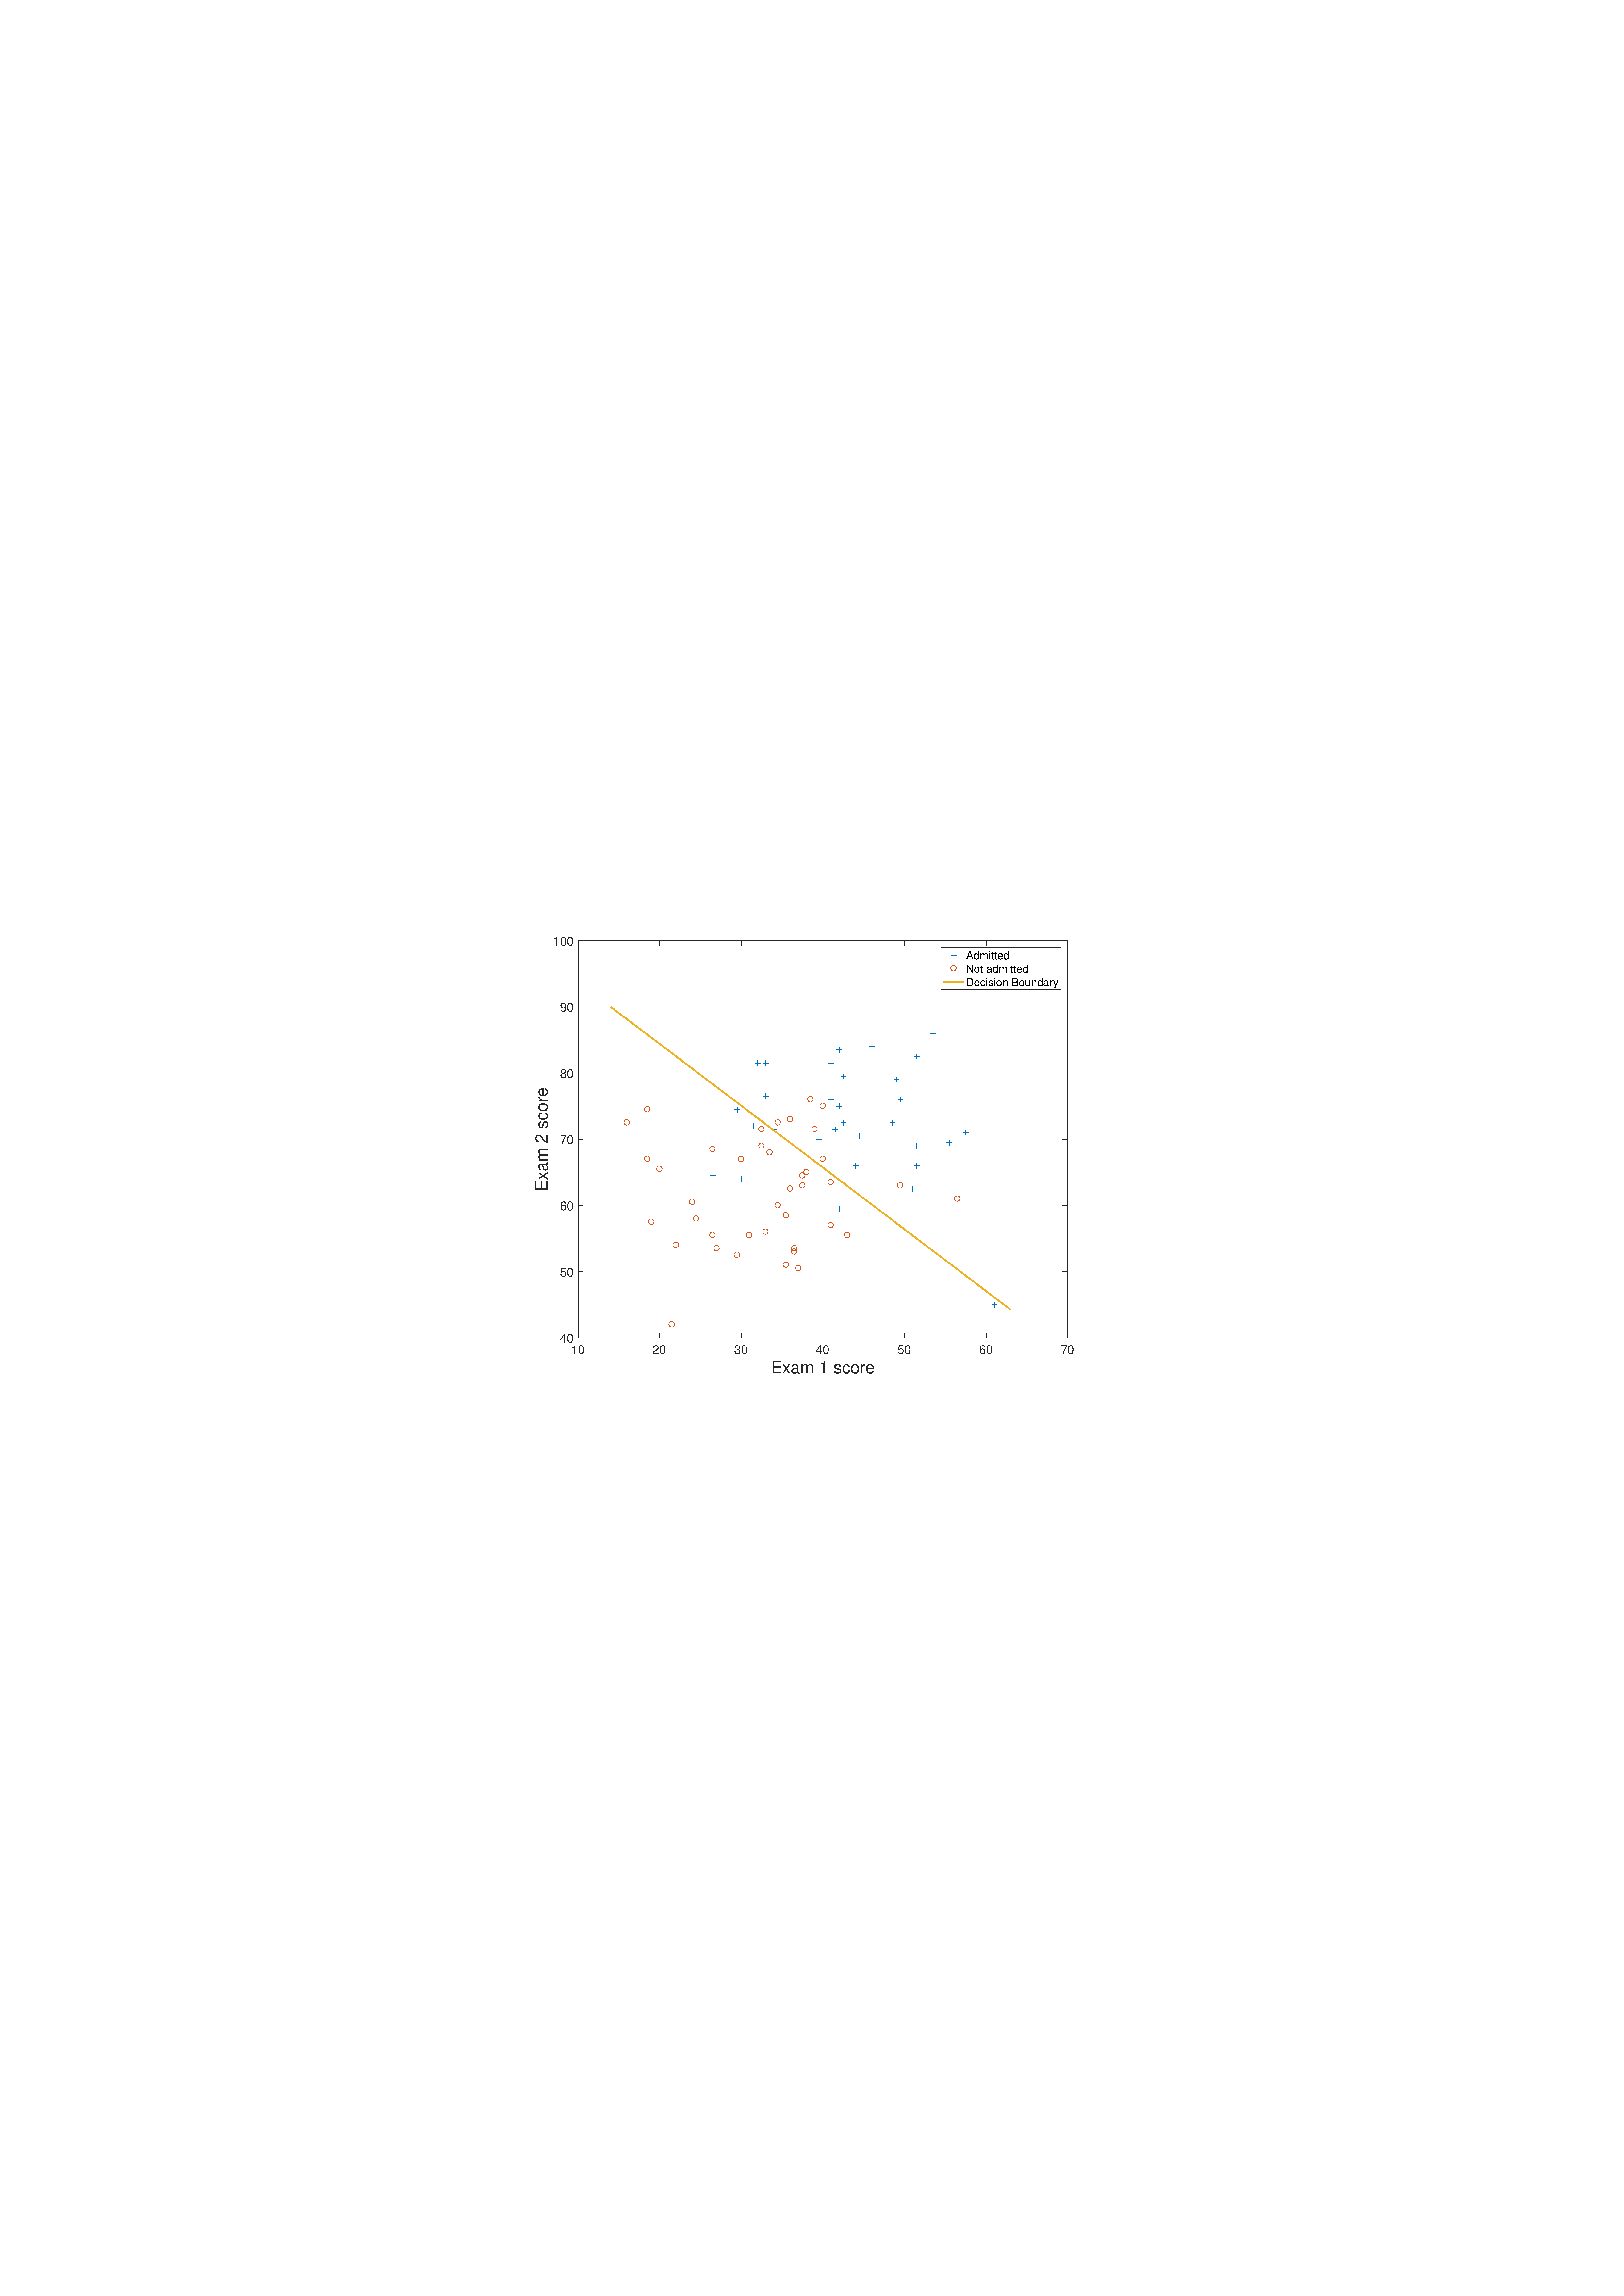
\includegraphics[width=.7\columnwidth]{regression}
    \end{figure}
    %
    \item What is the probability that a student with a score of 20 on Exam 1 and a score of 80 on Exam 2 will not be admitted?
    \end{enumerate}
    %


\section{Newton's Method}


  Our goal is to use Newton's method to minimize this function. Recall that the update rule for Newton's method is 
  %
  \begin{equation}
    \theta^{(t+1)}=\theta^{(t)}-H^{-1}\nabla_{\theta}L \nonumber
  \end{equation}  
  %
  In logistic regression, the Hessian is 
  %
  % \begin{equation}
  %   \nabla_{\theta}L = \frac{1}{m}\sum_{i=1}^{m}(h_{\theta}(x^{(i)})-y^{(i)})x^{(i)} 
  % \end{equation}  
  %
  \begin{equation}
    H = \frac{1}{m} \sum^m_{i=1} \left[ h_\theta(x^{(i)}) \left( 1 - h_\theta(x^{(i)}) \right) x^{(i)} \left(x^{(i)}\right)^T \right]
  \end{equation}  
  %
  Note that the formulas presented above are the vectorized versions. Specifically, this means that $x^{(i)} \in R^{n+1}$, $ x^{(i)}\left(x^{(i)}\right)^{T}\in R^{(n+1) \times (n+1)}$, while $h_{\theta}(x^{(i)})$ and $y^{(i)}$ are scalars.


  Now, implement Newton's method in your program, starting with the initial value of  $\theta = \vec{0}$. Use the same stopping condition (\ref{eq:stop}) as the gradient descent method. To determine how many iterations to use, calculate $L(\theta)$ for each iteration and plot your results. Newton's method often converges in 5-15 iterations. 

  



  \textbf{Finally, answer the following questions.}
  \begin{enumerate}
    \item What values of $\theta$ did you get when achieving convergence?
    \item Show how $L$ is decreased iteratively by Newton's method.
    \item Plot the decision boundary. 
    \item What is the probability that a student with a score of 20 on Exam 1 and a score of 80 on Exam 2 will not be admitted?
    \item What did you learn from comparing gradient descent method with Newton's method?
  \end{enumerate}






\end{document}
